%%%%%%%%%%%%%%%%%%%%%%%%%%%%%%%%%%%%%%%%%%%%%%
%                insertmeeting
% 1) Title (something creative & funny?)
% 2) Date (MM/DD/YYYY)
% 3) Location (ex. Hagerty High School)
% 4) People/Committees Present 
% 5) Picture 
% 6) Start Time & Stop Time (ex. 12:30AM to 4:30PM)
%%%%%%%%%%%%%%%%%%%%%%%%%%%%%%%%%%%%%%%%%%%%%%
\insertmeeting 
	{AprilTag for Signal Sleeve Detection} 
	{12/08/22}
	{Hagerty High School}
	{Anouska, Mohana, Ritam, Samantha}
	{Images/RobotPics/robot.jpg}
	{2:30 - 4:30}
	
\hhscommittee{Software}
\noindent\hfil\rule{\textwidth}{.4pt}\hfil
\subsubsection*{Goals}
\begin{itemize}
    \item Test diffrent signal sleeve variations

\end{itemize} 

\noindent\hfil\rule{\textwidth}{.4pt}\hfil

\subsubsection*{Accomplishments}
During the autonomous period, we need to detect the signal sleeve to determine our parking position. We wanted to be consisitent in detecting our signal sleeve. To do this, we tested multiple varaitions of signal sleeves. One variation insludes using QR codes as detectors. To detect these QR codes, we used software called AprilTag devloped by the APRIL lab at the University of Michigan. This code allows us to detect the 3D position, orientation, and identity of the tags. Although we thought this would increase our consistency and accuracy of detecting the tags, it actually did not make a diffrence. It sometimes also provided complications as the software could not detect the QR codes as easily when the sleeve was not placed in the correct orientation each time. This is why we chose to test other varaitions of sleves and discard the AprilTag Idea. 

\begin{figure}[htp]
\centering
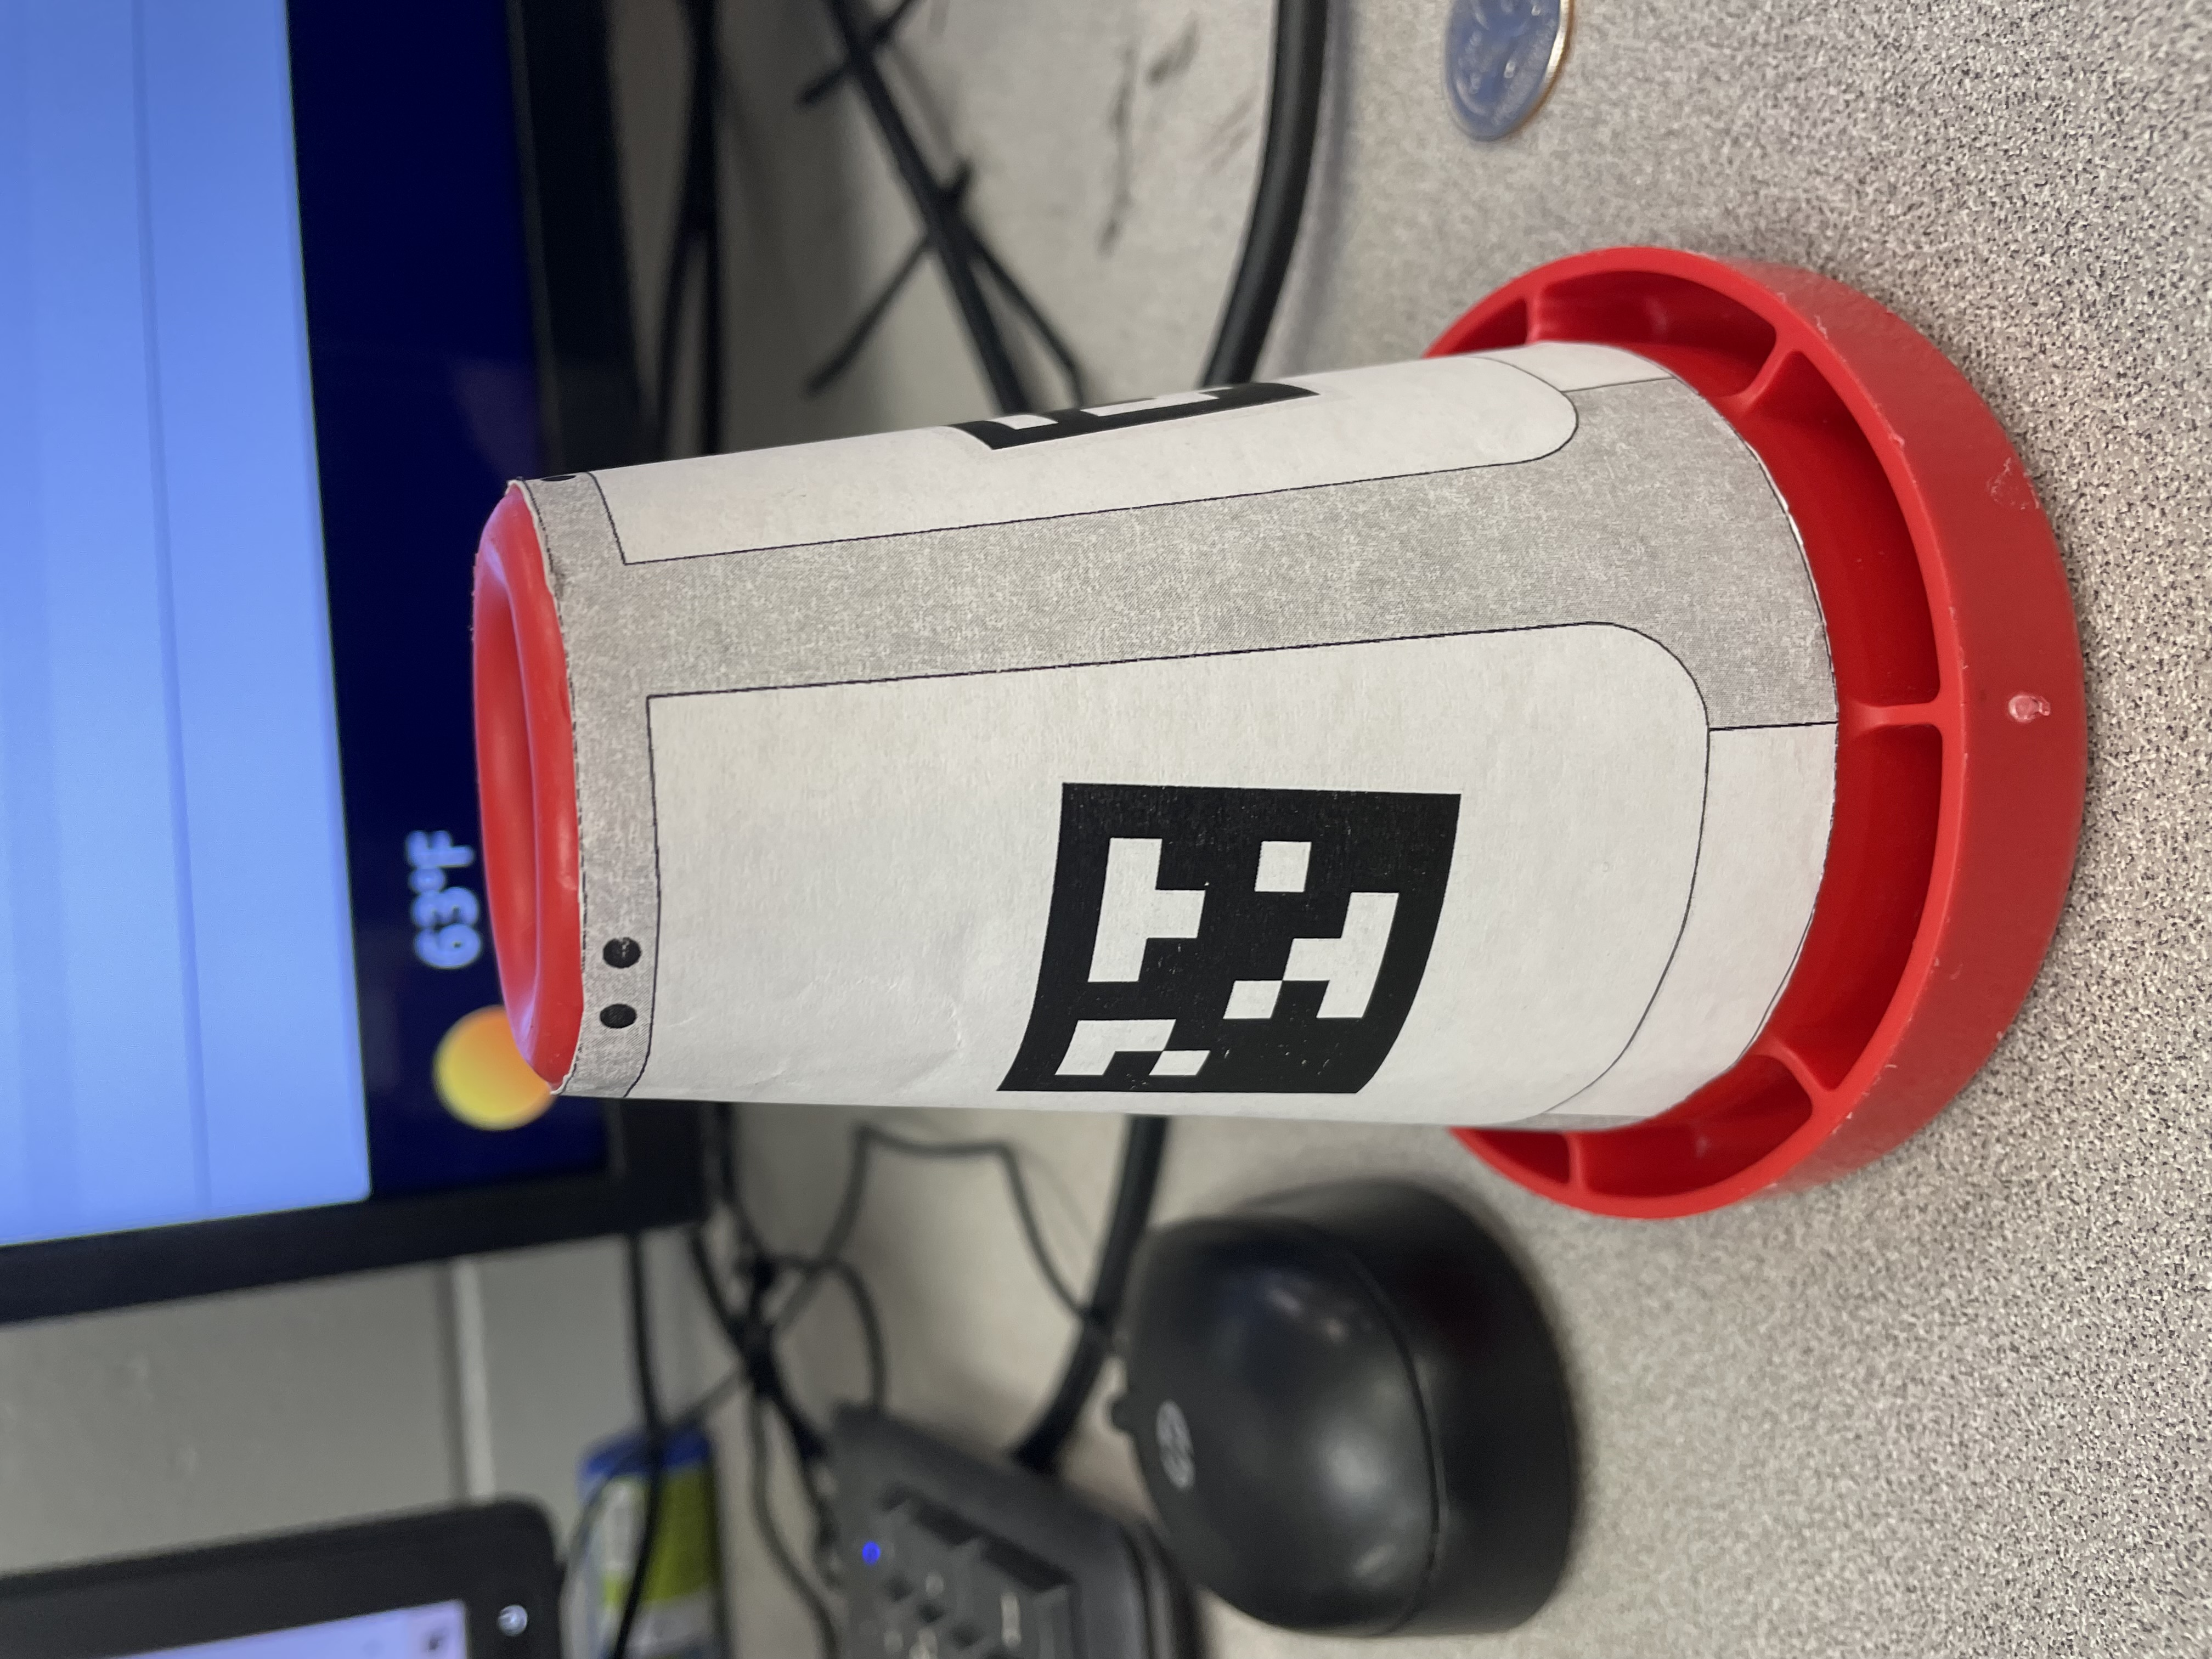
\includegraphics[width=0.9\textwidth, angle=270]{Meetings/December/12-08-22/IMG_4530.jpg}
\caption{April Tag on cone}
\label{fig:082322}
\end{figure}



\whatsnext{
\begin{itemize}
    \item Work on vision for auto
	\item Continue testing vision sleeves

\end{itemize} 
}

